% GEM-PIC-RZ for free-electron lasers: manuscript draft (started 2026-10-18)
% Compile: pdflatex gempic_fel && pdflatex gempic_fel
% Figures: python3 scripts/fig_emission.py, fig_fel.py, fig_averaging.py (data in ../benchmarks/harmonics, ../benchmarks/high_rho)
% Status and open items: NOTES.md
\documentclass[aps,prab,reprint,floatfix,superscriptaddress,amsmath,amssymb]{revtex4-2}

\usepackage{graphicx}
\usepackage{bm}
\usepackage{booktabs}
\usepackage{xcolor}
\usepackage[colorlinks=true,linkcolor=blue,citecolor=blue,urlcolor=blue]{hyperref}

\newcommand{\dd}{\mathrm{d}}
\newcommand{\todo}[1]{\textcolor{red}{[#1]}}

\begin{document}

\title{First-principles simulation of free-electron lasers with the Galilean electromagnetic particle-in-cell method:\\ even harmonics of planar undulators}

\author{Alexander Pukhov}
\affiliation{Institut f\"ur Theoretische Physik I, Heinrich-Heine-Universit\"at D\"usseldorf, 40225 D\"usseldorf, Germany}

\date{\today}

\begin{abstract}
Free-electron laser (FEL) codes average the electron motion over the undulator period and add the radiation harmonics through on-axis coupling factors. This is accurate for the fundamental, but the even harmonics of a planar undulator, which vanish on the axis, are not modelled at all. We show that the Galilean electromagnetic particle-in-cell method (GEM-PIC), which resolves the radiation carrier without a Courant limit, simulates FELs from first principles on a workstation. \todo{cost vs time-dependent GENESIS: measure before claiming.} The quasi-cylindrical code GEM-PIC-RZ reproduces the coherent spontaneous emission of a planar undulator in every azimuthal mode to within 2\,\% of the radiation integral and seeded amplifiers to within a few per cent of GENESIS. In a seeded planar FEL at 10.6\,nm it predicts a second harmonic of 10\,MW at saturation, $10^{-3}$ of the fundamental, where the averaged code computes none. \todo{one more sentence once the independent check (Puffin) or the LPA case is in}
\end{abstract}

\maketitle

%---------------------------------------------------------------------------
\section{Introduction}\label{sec:intro}

\todo{Draft. Message: averaged codes are excellent for the fundamental and the odd harmonics; what they leave out by construction is the even harmonics (and everything that depends on the transverse structure of the emission at harmonics). GEM-PIC gets them from first principles at moderate cost.}

High-gain free-electron lasers (FELs) produce coherent radiation from the terahertz range to hard X-rays~\cite{Pellegrini2016,KimHuangLindberg}. Their design relies on simulation codes such as GENESIS~1.3~\cite{Reiche1999,Genesis4}, which solve the coupled electron and radiation equations after two reductions: the electron motion is averaged over the undulator period, and the radiation is described by a slowly varying envelope at the resonant wavelength $\lambda_r$ and its harmonics. The averaging is the standard and well-tested model of the FEL interaction, valid when the gain per period is small, $\rho \ll 1$, with $\rho$ the Pierce parameter~\cite{Bonifacio1984}. Harmonics enter through coupling factors computed on the undulator axis, the Bessel-function factors $[JJ]_h$ of a planar undulator.

Some physics lies outside this model. In a planar undulator the odd harmonics radiate on the axis, the even harmonics do not: their coupling to an on-axis electron vanishes, and they are driven by the transverse gradient of the bunched beam. Averaged codes therefore omit them; GENESIS~4, for example, skips the source term of even harmonics altogether. Nonlinear harmonic generation in high-gain FELs, in which the fundamental bunching drives harmonic bunching and radiation, has been analysed theoretically~\cite{Huang2000,Freund2000} and observed experimentally~\cite{Tremaine2002}. \todo{check Freund2000, Tremaine2002; add Biedron et al. (APS LEUTL) if confirmed}

Codes that keep the electron motion within the period exist. Puffin solves the three-dimensional FEL equations without period averaging and without the slowly varying envelope approximation~\cite{Campbell2012}; full electromagnetic PIC codes such as MITHRA~\cite{Fallahi2018} solve Maxwell's equations directly, usually in a Lorentz-boosted frame to make the scale ratio between the undulator period and the radiation wavelength tractable~\cite{Vay2007}. \todo{WarpX/boosted-frame FEL references.} Full PIC is bound by the Courant condition on the radiation wavelength.

The Galilean electromagnetic particle-in-cell method (GEM-PIC)~\cite{GEMPIC} removes this limit. It writes Maxwell's equations in the Galilean variables $\zeta = z - ct$ and a slow coordinate $s$, keeps the slow derivative of the forward field, which therefore resolves its carrier, and needs no Courant condition because the field update is semi-implicit. GEM-PIC is not a quasi-static approximation: the forward radiation propagates, diffracts and is amplified with its carrier resolved. It was developed for laser-plasma accelerators~\cite{GEMPIC,GEMPICRZ_paper}; the same equations describe a beam that radiates in an undulator. The step in $s$ resolves the undulator period, the $\zeta$ grid the radiation wavelength. There is no period averaging, no envelope and no harmonic model: the electrons follow their orbits in the undulator and the fields of the beam, including its space charge, are computed in full.

In this paper we use the quasi-cylindrical code GEM-PIC-RZ~\cite{GEMPICRZ_paper,GEMPICRZ} to establish this approach for FELs. Section~\ref{sec:model} summarizes the model and the FEL-specific numerics. Section~\ref{sec:modes} shows that the harmonics of a planar undulator separate by azimuthal mode, which makes them natural to compute in a mode code. Section~\ref{sec:valid} validates the code: the coherent spontaneous emission against the radiation integral, mode by mode, and seeded and self-amplified FELs against GENESIS and scaling laws. Section~\ref{sec:harm} presents a seeded planar FEL with its second and third harmonics, and Sec.~\ref{sec:averaging} asks when period averaging itself becomes inaccurate. \todo{Sec. on LPA-driven FEL / superradiance, if included.}

%---------------------------------------------------------------------------
\section{Model}\label{sec:model}

\todo{Short: the equations are in Refs.~\cite{GEMPIC,GEMPICRZ_paper}; here only what matters for FELs.}

\emph{Fields.} GEM-PIC-RZ expands the fields in azimuthal modes, $F = F_0 + 2\,\mathrm{Re}\sum_{m=1}^{M} F_m e^{im\varphi}$, and combines the transverse fields into the forward components $R = E_\perp \pm B_\perp$ and the backward components $L$. The forward field obeys $\partial_s R = \ldots - j_\perp$ with the slow coordinate $s = z$ (GT2); it carries the FEL radiation, which stays at fixed $\zeta$ while the electrons slip back by $\lambda_r$ per period. $L$, $E_z$ and $B_z$ follow from their $\zeta$-equations at each level~\cite{GEMPICRZ_paper}. A level $s$ is the plane $z = s$ of the laboratory, so the beam particles at one level all sit at the same undulator phase.

\emph{Electrons.} Beam particles are advanced in $s$ with the Vay pusher~\cite{Vay2008} in the self-fields and the undulator field, $B_y = B_0 g(z)\cos k_u z$ (planar) or $(B_x, B_y) = B_0 g(z)(\cos k_u z, \sin k_u z)$ (helical), with linear entrance and exit ramps $g(z)$ of one period. Two corrections make the coupling exact to second order in the step $\Delta z$~\cite{GEMPICRZ}: the undulator kick of a step is multiplied by $\mathrm{sinc}(k_u\Delta z/2)$, the exact average of the field over the step, so that the orbit amplitude $K/\gamma$ and therefore the resonance are independent of $\Delta z$; and the transverse current is deposited with the velocity at the time of the position, completing the half step of the leapfrog with the undulator field. Without them the gain length depended on $\Delta z$ to first order. \todo{quantify: 9.5 $\to$ 8.3\,cm at 10\,nm.}

\emph{Self-fields and noise.} A bunch starts with its co-moving field for $\beta < 1$, so the longitudinal and transverse space charge are present from the start. Shot noise is loaded with the beamlet method of Fawley~\cite{Fawley2002}: beamlets of $N_b$ macroparticles at equally spaced phases are quiet for the harmonics $h < N_b$, and their displacements reproduce the bunching $\langle|b_h|^2\rangle = 1/N_e$ of $N_e$ random electrons.

\emph{Diagnostics.} The radiated power at harmonic $h$ is measured by demodulating each mode of $R$ and $L$ at $\pm h k_r$ over slices of a whole number of $\lambda_r$, which removes the fields that move with the beam; the Poynting flux of mode $m \ge 1$ is $\pi\int(|R_m|^2 - |L_m|^2)\,r\,\dd r$ (summed over the $r$ and $\varphi$ components), half of that for $m = 0$. The bunching $|\langle e^{ihk_r\zeta}\rangle|$ is computed per slice.

%---------------------------------------------------------------------------
\section{Harmonics and azimuthal modes}\label{sec:modes}

In a planar undulator, $x(t + T_u/2) = -x(t)$ and $y = 0$ along the orbit, with $T_u$ the period of the motion. Rotating the transverse plane by $\pi$ maps the orbit onto itself shifted by half a period; the radiation at harmonic $h$ acquires the factor $(-1)^h$ from the time shift. In cylindrical components the rotation only shifts $\varphi$ by $\pi$, so it multiplies a field of azimuthal mode $m$ by $(-1)^m$. Hence
\begin{equation}
\text{odd harmonics} \to \text{odd } m, \qquad \text{even harmonics} \to \text{even } m .
\end{equation}
The fundamental and the odd harmonics have an on-axis component in $m = 1$; the even harmonics radiate in $m = 0, 2, \ldots$ and vanish on the axis. For the lowest even-harmonic mode, $E_x \propto x\,f(r)$, the decomposition is $E_r = \tfrac12 r f(1 + \cos 2\varphi)$, $E_\varphi = -\tfrac12 r f \sin 2\varphi$: equal power in $m = 0$ and $m = 2$. A mode code with $M = 2$ thus contains the second harmonic completely, and the relation $P_{m=0} = P_{m=2}$ separates its radiation from the co-moving field of the $2k_r$ bunching, which also lives in $m = 0$. For a beam of finite length, with entrance and exit ramps, the separation holds per frequency band rather than exactly: a small even-mode part appears near $k_r$ (Fig.~\ref{fig:emission}).

%---------------------------------------------------------------------------
\section{Validation}\label{sec:valid}

\subsection{Coherent spontaneous emission at all harmonics}\label{sec:emission}

\emph{Why.} The radiation of a short bunch is the linear response of the field solver to a known current. Its comparison with the far-field radiation integral checks the coupling, the propagation and the mode structure of all harmonics at once, independently of any FEL code.

\emph{Setup.} A planar undulator of 10 periods ($\lambda_u = 10.67$\,mm, $K = 1$) and a bunch of 1\,fC at $\gamma = 100$ ($\lambda_r = 0.8\,\mu$m), with $\sigma_z = 20$\,nm and $\sigma_r = 5\,\mu$m, radiate coherently up to the third harmonic and to angles of $\sim 1.5/\gamma$. The reference is the radiation integral~\cite{Jackson} for the same trajectory (same field, ramps and no natural focusing) times the form factor $\exp(-k^2\sigma_z^2 - k^2\theta^2\sigma_r^2)$, decomposed into azimuthal modes of the far field. GEM-PIC-RZ uses $M = 3$, $\Delta\zeta = \lambda_r/64$, $\Delta z = \lambda_u/40$ and a radial grid from 0.5 to 25\,$\mu$m.

\emph{Results.} Figure~\ref{fig:emission} and Table~\ref{tab:emission} show the spectra and energies per mode. They agree to 0.3--1.8\,\%. The result is independent of $\Delta z$, $\Delta r$ and $\Delta\zeta$ to 0.5\,\% within factors of two. One condition matters: radiation emitted at angle $\theta$ advances in $\zeta$ by $\theta^2(L - z)/2$ over the rest of the undulator, 11\,$\mu$m at $\theta = 1.5/\gamma$ here, and the window must leave room for it ahead of the bunch. With only 1.3\,$\mu$m, modes 2 and 3 came out 12--14\,\% low.

\begin{figure}
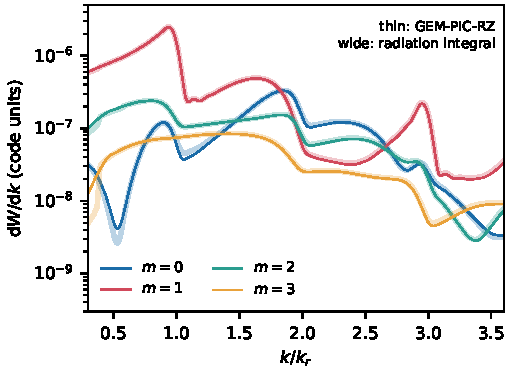
\includegraphics[width=\columnwidth]{figs/fig_emission.pdf}
\caption{Coherent spontaneous emission of a short bunch in a planar undulator (10 periods, $K = 1$, $\gamma = 100$): spectral energy per azimuthal mode, GEM-PIC-RZ (thin) and radiation integral (wide). Odd harmonics in odd modes, even harmonics in even modes.}
\label{fig:emission}
\end{figure}

\begin{table}
\caption{Coherent emission energy per azimuthal mode (code units, $1 = 2.94\times10^{-7}$\,J). The radiation integral has $9\times10^{-8}$ more in modes $m \ge 4$.}
\label{tab:emission}
\begin{ruledtabular}
\begin{tabular}{lccc}
mode & radiation integral & GEM-PIC-RZ & difference \\
\hline
$m = 0$ & $2.84\times10^{-7}$ & $2.79\times10^{-7}$ & $-1.8$\,\% \\
$m = 1$ & $1.361\times10^{-6}$ & $1.353\times10^{-6}$ & $-0.7$\,\% \\
$m = 2$ & $3.20\times10^{-7}$ & $3.19\times10^{-7}$ & $-0.3$\,\% \\
$m = 3$ & $1.346\times10^{-7}$ & $1.339\times10^{-7}$ & $-0.5$\,\% \\
\end{tabular}
\end{ruledtabular}
\end{table}

\subsection{High-gain amplifiers}\label{sec:helical}

\emph{Seeded, helical.} Two seeded amplifiers in helical undulators, at 10\,nm ($\gamma = 1000$, $\lambda_u = 1$\,cm, $K = 1$, 4\,kA, $\rho = 9.1\times10^{-3}$) and at 0.8\,nm ($\gamma = 5000$, $\lambda_u = 2$\,cm, $\rho = 2.9\times10^{-3}$), were compared with steady-state GENESIS~4~\cite{GEMPICRZ}. The power gain lengths are 8.33 and 38.7\,cm, against 7.92 and 38.4\,cm from GENESIS with the same physics: longitudinal space charge and the widening of the beam by its transverse space charge, which plain GENESIS omits (7.45 and 37.4\,cm). \todo{figure from benchmarks/genesis\_seeded (compare\_10nm.png) or a table only?}

\emph{SASE.} A compact SASE FEL (helical, $\gamma = 1000$, $\rho = 9\times10^{-3}$) started from the macroparticle noise gives a power gain length of 6.3 periods, against 6.4 periods from the Ming Xie fit~\cite{Xie1995}. \todo{redo with Fawley noise and a longer bunch; spectrum.}

%---------------------------------------------------------------------------
\section{Harmonics of a seeded planar FEL}\label{sec:harm}

\emph{Why.} This is the configuration in which an averaged code is incomplete by construction: the second harmonic of a planar undulator is not modelled.

\emph{Setup.} A planar undulator ($\lambda_u = 1$\,cm, $K = 1.5$, 100 periods, no natural focusing in either code) and a cold beam of 4\,kA at $\gamma = 1000$ with $\sigma_r = 10\,\mu$m give $\lambda_r = 10.625$\,nm and $\rho = 8.5\times10^{-3}$. A seed of 10\,MW ($w_0 = 30\,\mu$m) is polarized along the wiggle. GEM-PIC-RZ: $M = 2$, $\Delta\zeta = \lambda_r/32$, $\Delta z = \lambda_u/32$, a flat-top bunch of 1.9\,$\mu$m (179\,$\lambda_r$), longer than the slippage of 1.06\,$\mu$m; the radiation in the slices that met only the flat top is in the steady state and is compared with steady-state GENESIS~4 with fields at $h = 1, 2, 3$. The run took 1.8\,h on two CPU cores.

\emph{Results.} Figure~\ref{fig:fel} and Table~\ref{tab:fel}. The fundamental saturates at 10.4\,GW (GENESIS 9.8\,GW); the gain length is 13\,\% longer than in plain GENESIS, as in the helical case at 10\,nm, where it came from the space charge. The third harmonic reaches 2.1\,\% of the fundamental at saturation (GENESIS 2.8\,\%). \todo{3rd harmonic: run with $\Delta\zeta = \lambda_r/48$ and $M = 3$ to remove the resolution bias; post-saturation difference.}

Both codes bunch the beam at the second harmonic in the same way, with $b_2$ up to 0.5 before saturation. Only GEM-PIC-RZ radiates it. The second harmonic grows from the nonlinear bunching with a gain length of 5.3\,cm, about $L_g/1.5$, and reaches 9.6\,MW at saturation, $P_2/P_1 = 0.9\times10^{-3}$. Its power in $m = 0$ follows that in $m = 2$, as expected for the $E_x \propto x$ mode (Sec.~\ref{sec:modes}). \todo{transverse profile of the 2nd harmonic (zero on the axis) from the data files; comparison with Huang--Kim theory~\cite{Huang2000} and with Puffin.}

\begin{figure}
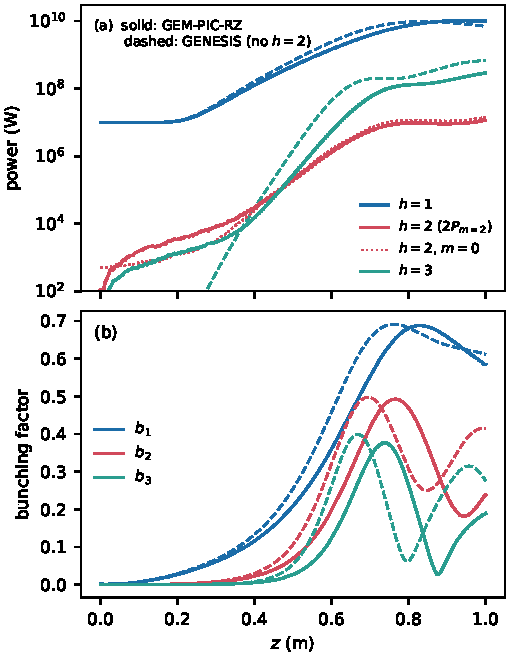
\includegraphics[width=\columnwidth]{figs/fig_fel.pdf}
\caption{Seeded planar FEL at 10.6\,nm: (a) power at the harmonics $h = 1, 2, 3$ and (b) bunching factors, GEM-PIC-RZ (solid) and GENESIS~4 (dashed), in the steady-state part of the bunch. GENESIS has no second-harmonic radiation.}
\label{fig:fel}
\end{figure}

\begin{table}
\caption{Seeded planar FEL at saturation.}
\label{tab:fel}
\begin{ruledtabular}
\begin{tabular}{lcc}
 & GENESIS 4 & GEM-PIC-RZ \\
\hline
saturation point & 0.84\,m & 0.94\,m \\
$P_1$ & 9.8\,GW & 10.4\,GW \\
power gain length & 7.0\,cm & 7.9\,cm \\
$P_2$ & 0 (not modelled) & 9.6\,MW \\
$P_3$ & 0.27\,GW & 0.22\,GW \\
$b_1$, $b_2$, $b_3$ & 0.66, 0.25, 0.13 & 0.63, 0.18, 0.14 \\
\end{tabular}
\end{ruledtabular}
\end{table}

\emph{Step size in planar undulators.} At $\Delta z = \lambda_u/16$, sufficient for the helical cases, the 4\,kA beam in the planar undulator blew up transversely from the tail forward (normalized emittance 2.8\,$\mu$m after 25 periods) and the gain length was 1.8 times too long. At $\lambda_u/24$, $/32$ and $/64$ the emittance after 25 periods was 0.13, 0.04 and 0.02\,$\mu$m, and the power at $\lambda_u/32$ and $/64$ agreed. Finer beam sub-steps or a second field iteration did not help, so the field step is the cause. \todo{Understand: candidate is the $s$-discretization of the large co-moving field of the oscillating transverse current $j_x \propto \cos k_u s$, whose $E + v\times B$ cancellation is broken at second order in $k_u\Delta z$; a fix would make $\lambda_u/16$ usable again.}

%---------------------------------------------------------------------------
\section{When does period averaging fail?}\label{sec:averaging}

\emph{Why.} A natural expectation is that unaveraged codes are needed when the gain per period is large, $\rho \gtrsim 0.01$, as in compact FELs driven by plasma accelerators~\cite{Wang2021,Labat2023,Pompili2022}. We tested this in one dimension.

\emph{Model.} The steady-state 1D FEL equations of a planar undulator were integrated (RK4, 96 steps per period, 256 particles per bucket) in two forms: the averaged equations with the coupling $K[JJ]/2$ and the mean longitudinal velocity, and the unaveraged equations with $v_x = cK\cos(k_u z)/\gamma$ and the figure-eight oscillation of $v_z$, the field remaining a single-frequency slowly varying amplitude.

\emph{Results.} Figure~\ref{fig:averaging}: both reproduce $L_{g,1D} = \lambda_u/(4\pi\sqrt3\rho)$ and $P_\mathrm{sat} = 1.36\rho P_b$ for $\rho \to 0$. Up to $\rho = 0.15$, where the field grows $e$-fold in a third of a period, the gain lengths differ by less than 3\,\%, independently of $K$; the saturation power of the averaged model is low by about $1.2\rho$ (5\,\% at $\rho = 0.04$). Period averaging is therefore not the main limitation of averaged codes even at large $\rho$; what they omit are the even harmonics and the full space-charge and radiation fields. \todo{Time-dependent version: superradiant spikes and short bunches, where the slice and slippage model may matter more.}

\begin{figure}
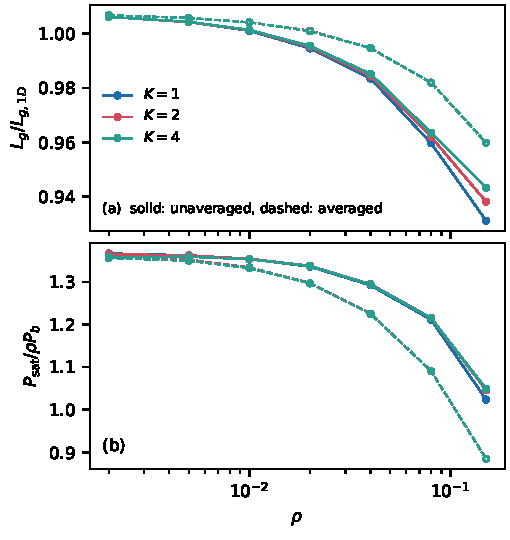
\includegraphics[width=\columnwidth]{figs/fig_averaging.pdf}
\caption{1D steady-state planar FEL with averaged (dashed) and unaveraged (solid) electron motion: (a) power gain length and (b) saturation power, against $\rho$.}
\label{fig:averaging}
\end{figure}

%---------------------------------------------------------------------------
\section{Discussion and outlook}\label{sec:disc}

\todo{Cost: GEM-PIC-RZ 1.8\,h on 2 cores for 100 periods and a 1.9\,$\mu$m flat top vs GENESIS steady state 30\,s (one slice) and GENESIS time-dependent (to be measured). Limits: no backward wave (L is computed from its $\zeta$ equation, i.e. its slow derivative is dropped); $\lambda_r$ resolved in $\zeta$; azimuthal mode truncation; transverse space charge always present. Outlook: plasma accelerator + transport + FEL in one code (combined run planned); superradiance; harmonics with orbital angular momentum in helical undulators; Puffin / MITHRA comparison.}

%---------------------------------------------------------------------------
\section{Conclusions}\label{sec:concl}

\todo{to write}

\begin{acknowledgments}
\todo{funding; computing time.} Parts of the code and of the analysis were developed with the assistance of the AI model Claude~\cite{Claude}.
\end{acknowledgments}

\begin{thebibliography}{99}
\bibitem{Pellegrini2016} C. Pellegrini, A. Marinelli, and S. Reiche, The physics of x-ray free-electron lasers, Rev. Mod. Phys. \textbf{88}, 015006 (2016).
\bibitem{KimHuangLindberg} K.-J. Kim, Z. Huang, and R. Lindberg, \textit{Synchrotron Radiation and Free-Electron Lasers} (Cambridge University Press, Cambridge, 2017).
\bibitem{Reiche1999} S. Reiche, GENESIS 1.3: a fully 3D time-dependent FEL simulation code, Nucl. Instrum. Methods Phys. Res., Sect. A \textbf{429}, 243 (1999).
\bibitem{Genesis4} S. Reiche, GENESIS 1.3 version 4, \url{https://github.com/svenreiche/Genesis-1.3-Version4} \todo{version used, citable reference}.
\bibitem{Bonifacio1984} R. Bonifacio, C. Pellegrini, and L. M. Narducci, Collective instabilities and high-gain regime in a free electron laser, Opt. Commun. \textbf{50}, 373 (1984).
\bibitem{Huang2000} Z. Huang and K.-J. Kim, Three-dimensional analysis of harmonic generation in high-gain free-electron lasers, Phys. Rev. E \textbf{62}, 7295 (2000).
\bibitem{Freund2000} H. P. Freund, S. G. Biedron, and S. V. Milton, Nonlinear harmonic generation in free-electron lasers, IEEE J. Quantum Electron. \textbf{36}, 275 (2000). \todo{check}
\bibitem{Tremaine2002} A. Tremaine \textit{et al.}, Experimental characterization of nonlinear harmonic radiation from a visible self-amplified spontaneous emission free-electron laser at saturation, Phys. Rev. Lett. \textbf{88}, 204801 (2002). \todo{check}
\bibitem{Campbell2012} L. T. Campbell and B. W. J. McNeil, Puffin: a three dimensional, unaveraged free electron laser simulation code, Phys. Plasmas \textbf{19}, 093119 (2012).
\bibitem{Fallahi2018} A. Fallahi, A. Yahaghi, and F. X. K\"artner, MITHRA 1.0: a full-wave simulation tool for free electron lasers, Comput. Phys. Commun. \textbf{228}, 192 (2018).
\bibitem{Vay2007} J.-L. Vay, Noninvariance of space- and time-scale ranges under a Lorentz transformation and the implications for the study of relativistic interactions, Phys. Rev. Lett. \textbf{98}, 130405 (2007).
\bibitem{GEMPIC} A. Pukhov, N. Elkina, and T. Wilson, Galilean electromagnetic particle-in-cell code, \href{https://doi.org/10.1016/j.jcp.2026.115331}{J. Comput. Phys. \textbf{567}, 115331 (2026)}.
\bibitem{GEMPICRZ_paper} A. Pukhov, GEM-PIC-RZ: a Galilean electromagnetic particle-in-cell code in quasi-cylindrical geometry with nonuniform grids, \todo{arXiv number}.
\bibitem{GEMPICRZ} A. Pukhov, GEM-PIC-RZ, \url{https://github.com/AlexMPukhov/GEM-PIC-RZ} (2026); benchmarks in \texttt{benchmarks/}.
\bibitem{Vay2008} J.-L. Vay, Simulation of beams or plasmas crossing at relativistic velocity, Phys. Plasmas \textbf{15}, 056701 (2008).
\bibitem{Fawley2002} W. M. Fawley, Algorithm for loading shot noise microbunching in multidimensional, free-electron laser simulation codes, Phys. Rev. ST Accel. Beams \textbf{5}, 070701 (2002).
\bibitem{Jackson} J. D. Jackson, \textit{Classical Electrodynamics}, 3rd ed. (Wiley, New York, 1999).
\bibitem{Xie1995} M. Xie, Design optimization for an X-ray free electron laser driven by SLAC linac, in \textit{Proc. PAC'95} (IEEE, 1995), p.~183.
\bibitem{Wang2021} W. Wang \textit{et al.}, Free-electron lasing at 27 nanometres based on a laser wakefield accelerator, Nature \textbf{595}, 516 (2021).
\bibitem{Labat2023} M. Labat \textit{et al.}, Seeded free-electron laser driven by a compact laser plasma accelerator, Nat. Photon. \textbf{17}, 150 (2023).
\bibitem{Pompili2022} R. Pompili \textit{et al.}, Free-electron lasing with compact beam-driven plasma wakefield accelerator, Nature \textbf{605}, 659 (2022).
\bibitem{Claude} Anthropic, Claude, large language model (model \texttt{claude-opus-5-5}), \url{https://www.anthropic.com/claude}, used in October 2026.
\end{thebibliography}

\end{document}
